\chapter{Results}
\label{ch:Results}

\section{Challenges evaluating XAI Explanations}

As we've seen in the previous chapter, shap is a very specific recently proposed method to generate an explanation. Its algorithm follows rules and gives a result which exactly matches the output from the classifier \cite{NIPS2017_7062}.

\begin{quote}{Scott M. Lundberg, Su-In Lee \cite{shapPaper}}
    When approximating the original model $f$ for a specific input $x$, local accuracy requires the explanation model to at least match the output of f for the [\textit{original input $x$}]
\end{quote}

Even if, using \textit{kernelexplainer}, the result is approximated, this approximation error is not directly accessible, because competitive game theory produces a feature value which when all feature values are summed up, exactly matches the classification result \cite{shapPaper, compGameTheory}. Nonetheless there are multiple possibilities to evaluate the quality of an explanation.

\section{Dimensions of the explanation quality}

I propose to categorize explanation qualities into three categories: \textbf{Accuracy, Interpretability} and \textbf{Resource-requirements.} These are not independent, we expect accuracy to increase with more allocated computational resource and vice-versa. Interpretability, \textit{meaning the ease with which the result can be understood} is expected to be negatively correlated with the accuracy. The more features that are analyzed and presented to the data analyst, the more difficult it gets to interpret the explanation.

It is important to keep those interactions in mind when tweaking parameters of the explanations. A definitive advice on how to set those parameters will not be possible because it is unclear how important each dimension is for the user.

In this thesis we will not be able to tackle all of these dimensions and will focus on the accuracy and interpretability ones.

\section{Necessary characteristics to analyse XAI results}

The principle is simple, we've seen above that to evaluate an explanation we need to compare it to another explanation to get useful results. Following properties need to be fulfilled for an evaluation method to be of worth:

\begin{enumerate}
    \item Be able to generate a theoretically unlimited amount of explanations for each parameter tweak.
    \item Be able to pinpoint the influence of a single parameter (or a clear defined combination of multiple parameters).
    \item Be able to theorize about the results on a \textbf{global} level (See \autoref{fig:ShapExplEx1}), \textit{meaning that the influence of tweaking one or multiple parameters can be logically understood or at least theorized about by looking at a multitude of explanations}. \textit{If the tweaking of a parameter results in chaotic changes which are not understood, tweaking that parameter is pointless}.
    \item \textit{(optional but desirable)} Be able to theorize about the results on a \textbf{local} level, \textit{by looking at a tuple of explanations of a single corpus with different parameters.}
\end{enumerate}

While the first three points are rather obvious, the last one might be a bit controversial and I will try to explain my reasoning. The goal of text-explanations is mostly to debug classifiers, to understand where they are failing and to fix issues in the underlying data. Examples like biased data, inadvertently pre-classified data (see \autoref{section:ExplanationExample}) come to mind. These issues are not always visible on a global scale. A lot of times the classifier uses shortcuts like detecting email-providers only on certain data entries which will not be visible when looking at a multitude of explanations. Some issues will not be detectable on a global approach, so explanations should not only focus on the entirety of the data-set. Since this is the expected use case for someone implementing/using shap, tweaking parameters of his implementation to learn more about a classification issue in a single classification is an important use case and it would be desirable that tweaking a parameter has an immediate effect on this single classification. This will be discussed in more detail in \autoref{ch:outlook}.


\section{Parameter: Text hierarchy}

One important parameter we will evaluate is the text-hierarchy, defining which entries shap considers atomic entities \textit{(which cannot be divided)}. This is important, because the user can only process a limited amount of information at once \cite{Baecker2014}, but the length of that information plays a secondary role, as long as each chunk of information is perceived as one \cite{Fountain2012}.

\subsection{Dataset}

The dataset used to generate these results, is a collection of christian/atheism themed emails provided by the Newsgroups20 \cite{Newsgroups20} dataset. It is composed of 717 emails. We fitted a binary tfidf classifier for each text hierarchy supposedly classifying the emails in atheist and christian categories. Using the 80/20 rule (80\% training data, 20\% test data) our classifiers never dipped below 90\% accuracy on any of our analyses (they are refitted on each run). The dataset and our approach is not ideal though, and can rightfully be criticized which we try to do in \autoref{sec:critique}.

\subsection{Context importance by text hierarchy}


\begin{table}[H]
    \centering
    \begin{tabular}{c|c}
         \textbf{Text-Hierarchy} & \textbf{Regex}\\ \hline
         Word & \verb/\b[\w|'|-]+\b/ \\
         Sentence & \verb/[^(.|?|!|\n)]+/ \\
         Paragraph & \verb/((?:[^\n][\n]?)+)/ \\
         2-gram & \verb/\b[\w|'|-]+\b\W+\b[\w|'|-]+\b/ \\
         ... & ...
    \end{tabular}
    \caption{Text Hierarchies}
    \label{tab:textHierarchies}
\end{table}

We will now try to evaluate the explanation results by evaluating the Newsgroup20 \cite{Newsgroups20} dataset with different text-hierarchies. For that purpose we used following formula:

\noindent\rule[0.5ex]{\linewidth}{1pt}

\textbf{\begin{multline}
\label{contextEvalFormula}
\mathrm{contextInfluence}(w’) = \\
| (\mathrm{classificationScore}(W)- \mathrm{classificationScore}(W\backslash w')) - \mathrm{shapFeatureImportance}(w') |
\end{multline}}

\textit{$w'$: The feature which had the most impact in the classification according to shap} \\
\textit{$contextInfluence(w')$: The importance of the context of the word w' according to shap} \\
\textit{$classificationScore(W)$: The classification score the classifier gives the text W}\\
\textit{$classificationScore(W \backslash w')$: The value the classifier gives the text W without the word w'}\\
\textit{$shapFeatureImportance(w')$: The feature importance shap gives the word w'}

\noindent\rule[0.5ex]{\linewidth}{1pt}
\vspace{1cm}

In \autoref{contextEvalFormula} we compare the change of the classification score when we remove the feature w' with the feature importance shap gives w'. We averaged the context influence over the entire corpus. We repeated this but instead of only remove a single feature we removed multiple features (in descending feature importance order) at once and plotted these results in \autoref{fig:shapEvalResults}.


\begin{figure}[H]
\centering
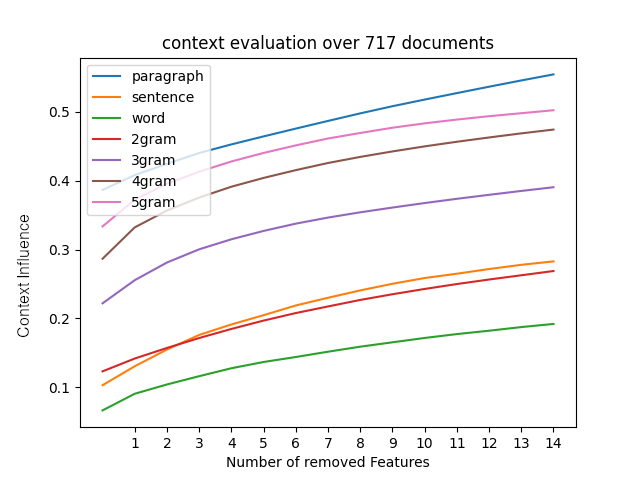
\includegraphics[width=\linewidth]{images/06_results/clemensEvalPlotAllSelectedDocsCombinedYAXIS.png}
\caption{Shap Evaluation Results.}
\label{fig:shapEvalResults}
\end{figure}

Now let's analyze what we did here. Calculating the importance of a feature by re-classifying the text without said feature is a simple perturbation based approach used before frameworks like \textit{lime} and \textit{shap} were developed. It does not take in account the context of a feature, an issue most recent approaches try to fix. The shap algorithm uses that method as well but adds more steps to it with the goal to \textbf{include the importance of the context} (\autoref{section:compGameTheory}), and to a smaller degree, make the explanation more intuitive (\autoref{section:shapleyProp}). So what \textbf{we are evaluating is how much weight the context of features has depending on the text hierarchy.}
\vspace{1cm}

With that information, let's analyze the produced plot:
\begin{itemize}
    \item As expected, generally, the bigger the group of text taken out of the original email, the more dependent it is of its respective context. This is what we would expect because each word can interact with other words in the text.
    \item This rule is however broken for sentences. A sentence has 14 words on average. Since we are working with emails, a sentence might be shorter. Nonetheless we would expect the contect influence to hover above the 5gram curve.
    \item The same could be said about paragraphs, meaning they hold multiple sentences and are just slightly more dependent on the context than 5grams. I would be careful though, the original dataset being emails, did not provide very structured paragraphs. Furthermore, I consider emails to be too short to draw any decisive conclusion about paragraphs based on our results.
\end{itemize}



The fact that sentences are less dependent on their context than any other random n-gram makes sense, they are, from a grammatical standpoint, a self contained part of the text. On average, it is much less dependent on its context than a string of words of the same length cutting in half two sentences (as shown in our analysis). Even though our findings are unspectacular, they allow us to substantially improve the quality of XAI text explainers. The goal of an explainer is to provide as much information as possible without overwhelming the user. \textbf{We can, instead of providing words to the user, provide entire sentences}, which massively increases the quality of the explanation (because of the reduced context importance) without overwhelming him with to much information. As a reminder, chunking allows the human brain to process sentences with n words much faster than n independent words \cite{ChunkingWikipedia}.

This is especially useful, if the previous explanation was not useful because the words provided were too dependent on their context (like shown in \autoref{section:ExplanationExample}). Our data shows that the per word influence of the context is reduced by 89,33 percent when comparing the context influence of sentences to the context influence of words.

\subsection{Critical analysis}
\label{sec:critique}

As mentioned before, there are a few points which could be improved in our approach, I will list them below:

\begin{enumerate}
    \item The emails are to short to analyse paragraphs properly. \textit{This is absolutely correct, in our analysis, we remove up to 15 features, and none of the emails in the dataset include over 15 paragraphs. The paragraph plot should not be used to make any conclusion and we only formulated a suggestion to use sentences, we did not make any statement about paragraphs.}
    \item Why not use the same classifier for each text hierarchy? \textit{Due to technical limitations, it was not possible to use the same classifier. \textit{Kernelexplainer} does not support text classifiers properly, during my time working on this thesis, the support for kernelexplainer was dropped due to a multitude of reasons. I can only support that decision from the shap development team, kernelexplainer was very difficult to work with, I do not recommend using it to anyone.}
    \item The dataset is too small. \textit{I agree with this statement, this was sadly due to time and technical limitations running the analysis on the institutes server takes multiple days. Substantially increasing the dataset size would have demanded code optimizations which would most likely have broken the modularity of the framework.}
    \item Where is the error bar? \textit{I would have liked to add an error bar to my work, but was asked to prioritize onto the framework. If you wish to verify my work, I invite you to write me an email, I will gladly provide the research data necessary. To get access to the code repository, please contact the \href{https://dbis.ipd.kit.edu/english/index.php}{Institute for Program Structures and Data Organization (IPD)}.}
\end{enumerate}